\section{Controlling the Virtual Rover}

In \fig\ref{fig:acc_model} we depict the top-level model of the controller for
follower vehicle. This model is a subset of the model used to control the
physical toy that has been abstractly described in
\sect\ref{sec:toy_rover_controller}. In particular, we have adapted the cruise
control functionality of the original model to implement a ``follow the leader''
behavior.

The controller is meant to function in a loop by reading the
\emph{Velocity} of the follower rover itself, the velocity of the leader rover
(input by the \textsf{VelocityFrontObstacle} signal) and the \textsf{Distance} to
the leader rover. By using these values it constantly updates the maximal
allowed acceleration (\textsf{MaxAcceleration}) as well as
the target velocity (\textsf{TargetVelocity}) for the follower rover.

The controller is composed by a number of \af components, as follows:
\begin{itemize}
  \item the \textsf{TargetDistance} component is responsible for calculating the
  ideal distance to the leader rover. This distance is proportional to the speed of
the leader, as larger speeds imply larger distances for breaking. 
  \item The \textsf{P Controller} component is a \pid controller for adjusting
  the the velocity of the follower in order to reach the target distance to the
leader.
\item The \textsf{TargetVelocityController} component decides whether the
\textsf{TargetVelocity} output should remain the same as in the previous step
(saved in the \textsf{MaxVelocityMemory}) or should be updated to the
\emph{TargetVelocityIn} calculated by the \textsf{P Controller} component.
\levi{don't understand this part of the model}
\end{itemize}

\begin{figure}[!h]
\centering
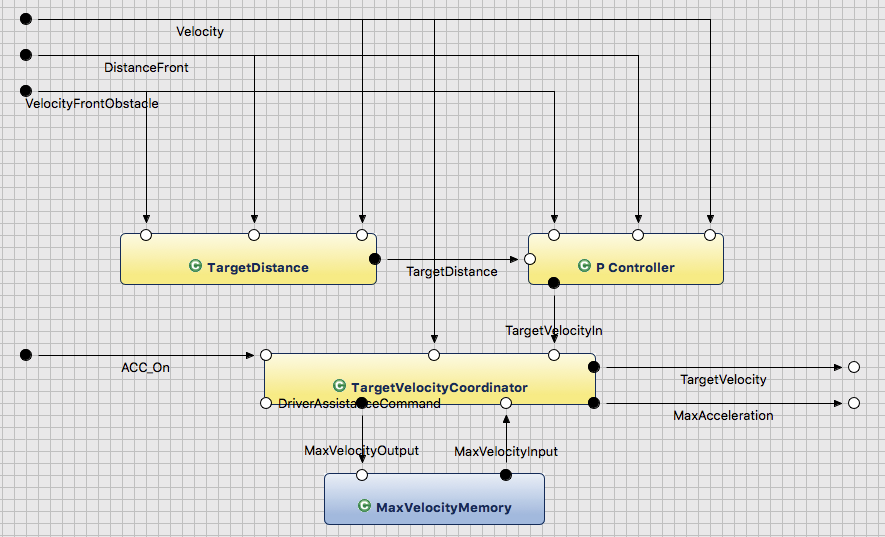
\includegraphics[width=1\textwidth]{images/ACC_controller_model.png}
\caption{The controller for the Automatic Cruise Control modelled in \af}
\label{fig:acc_model}
\end{figure}

The logic for the \emph{P Controller} is shown in \fig\ref{fig:pid_controller}
(in the \af action language which has Java-like syntax). The snippet of
code starts by checking whether the rover is already too close to the
leader, or the leader's speed is too low. In this case the
\textsf{TargetVelocity} is set to \textsf{0}, practically making the rover stop.
Otherwise a new \emph{TargetVelocity} is computed in order to reach the
\emph{TargetDistance}. The \emph{TargetVelocity} is calculated by multiplying
the \textsf{P} coeficient of the \pid controller by the difference between the
\emph{TargetDistance} and the distance to the leader rover. This formula
produces a new value for the current speed which corresponds to a positive or
negative increment to the current speed as read in by the \textsf{Velocity}
sensor.

Note that the \pid controller used by the \textsf{P Controller} is very simple,
and in fact no \textsf{I} (\emph{integral}, corresponding to the previous
experience) or \textsf{D} (\emph{derivative}, corresponding to the anticipated
value of speed given the current rate of change) are taken into consideration.

\begin{figure}[!h]
\centering
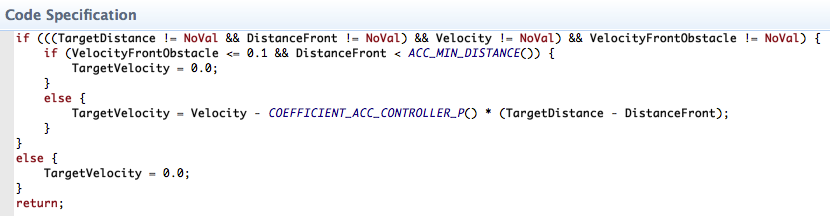
\includegraphics[width=1\textwidth]{images/code_spec_P_controller.png}
\caption{pid controller \af}
\label{fig:pid_controller}
\end{figure}

\begin{figure}[!h]
\centering
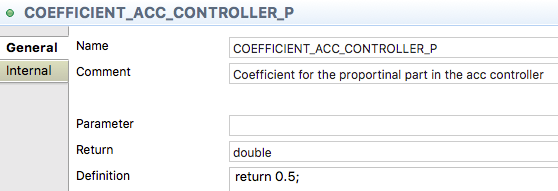
\includegraphics[width=.7\textwidth]{images/P_coefficient_controller.png}
\caption{P Coefficient}
\label{fig:p_coefficient}
\end{figure}